\chapter{Methodology}\label{C:method} 

\section{Selecting Languages}
The languages explored in this study include Java, C\#, JavaScript and Lua. These languages were were explored because they each have large enough open source communities to gather meaningful corpora of projects and between them they offer a wide range of native object inheritance model implementations. They also offer a helpful division between two languages with native support for classical inheritance object models and two languages with native support for delegation object models.
\newline

Java and C\# both offer native implementations of classical inheritance so can be used to analyse the frequency of use of patterns which surround this classical inheritance model. These languages also allow an analysis of patterns which would behave differently under a delegation object model, representing cases which could be difficult to reimplement in another language with different native support.
\newline

JavaScript and Lua both offer delegation natively so can provide a measure of how often developers are making use of these delegation features and also how often developers in these languages are choosing to ignore the languages' native features in favour of classical inheritance models.

\section{Assembling Corpora}
To analyse each language, we first needed to collect a corpus representative of that language's use in real world software development projects. In the case of Java, we adopted The Qualitas Corpus, which is a large collection of open source projects written in the Java language~\cite{QualitasCorpus}. Likewise, with JavaScript, we have adopted an existing corpus used by the team that developed JSClassFinder~\cite{JSClassFinder}.
\newline

For the other studied languages, Lua and C\#, quality existing corpora could not be found. For each of these languages, the top 25 open source projects were sourced from GitHub's ``Trending this month" list for June, 2016. This source was chosen because it provides a group of projects for each language which are in active development as measured by GitHub, and which are easy to access. This helps to ensure that the analysis performed will be as relevant as possible to modern software development.

\section{Static Analysis Tools}
The core of this empirical study is the analysis of corpora of code written in each of the investigated languages. This analysis makes use of many static code analysis methods including the following:
\begin{itemize}
	\item Grep is used to perform regular expression searches on files. This can detect some of the more simple patterns explored in this paper. More specifically, an implementation of Grep known as PCREGrep (Perl Compatible Regular Expression Grep) was used to allow multiline analysis which is a requirement of a source code corpus analysis.
	\item ANTLR (Another Tool For Language Recognition) is a tool which accepts a language grammar as input and produces a lexer and parser. This lexer and parser can then accept a file which conforms to the grammar definition and construct a syntax tree to represent that file.
	\item JSClassFinder is a tool which detects patterns indicative of class and method declarations in JavaScript projects. It accepts JSON representations of the syntax trees of JavaScript files as input and produces the Class Usage Ratio of the syntax tree as its output~\cite{JSClassFinder}.
	\item Esprima accepts a JavaScript code file as input and produces a JSON representation of the syntax tree of that file as output. This JSON file can then be used as the input to the JSClassFinder tool.
\end{itemize}
Each of these tools helps to extract valuable information from one of more of the languages analysed in this study.

\section{Java Analysis}
Finding occurrences of classical inheritance in Java is as simple as looking for the extends keyword with a ``Grep" regular expression search. Finding examples of delegation and forwarding is more difficult and requires more information about the syntax tree of the program. To achieve this, each program of the corpus was passed through ANTLR which parses each file according to a lexer and parser generated from a Java grammar. ANTLR then constructs an abstract syntax tree which can then be traversed to search for relevant patterns.
\newline

The process for analysing a Java project follows a pipeline structure where each file is parsed and analysed in isolation. The resulting statistics of each file are then aggregated to form the overall statistics across the projects. This file isolation is important because the syntax trees produced by ANTLR consume large amounts of memory so it is not possible to hold all the Java files for a project in memory simultaneously.
\newline

\begin{center}
	\captionof{figure}{Java Analysis Pipeline}
	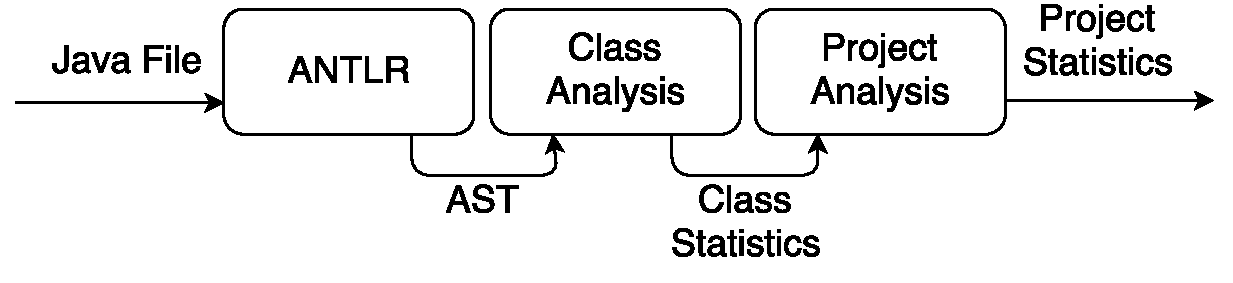
\includegraphics[scale=0.70]{AntlrPipeline.pdf}
\end{center}

\section{C\# Analysis}
As with Java, C\# was analysed using a lexer and parser generated by loading a C\# 6 grammar into ANTLR. The analysis for each project in the corpus was performed in three major passes:
\begin{enumerate}
	\item Use ANTLR, along with a C\# preprocessor grammar, to perform the first stage towards forming a syntax tree. This stage evaluates preprocessor directives in the program to ensure the remaining file can transformed into a well formed syntax tree. Included in this stage is the removal of \cs{\#region} tags and conditional directives which exclude and include blocks of source code based on boolean arguments.
	\item Use ANTLR, along with a C\# program grammar, to create a syntax tree for each C\# code file in the corpus and traverse it to find all class declaration subtrees. Collect these class declarations to be explored in later steps.
	\item Run a visitor down each class declaration subtree, searching for all the methods and recording their modifiers. A type hierarchy is also established at this step to allow classes to find information about method calls they make which may be dispatched to a method in their superclass.
	\item Run another visitor down each class declaration tree and find constructors and check which methods are called against the modifiers found in the previous pass to determine which methods could miss their intended target under a different object initialisation model.
\end{enumerate}
The statistics gathered for each file in each project were then aggregated across the corpus to collect information about the corpus as a whole.

\section{JavaScript Analysis}
In JavaScript, there are many ways developers make use of classical inheritance patterns despite the lack of native support in the language. This is largely a result of the numerous libraries which offer their own implementation of classical inheritance behaviour. Some examples of these patterns can be found in the following table:
\begin{center}
	\captionof{table}{JavaScript Patterns}
	\begin{tabular}{|p{5cm}|p{9cm}|}
		\hline
		\multicolumn{2}{|c|}{JavaScript}                                                                                                                                                                  \\ \hline
		Inheritance 1                  & \code{var a = function( b )\{    c.call ( this , d );\}}                                                                                      \\ \hline
		Inheritance 2                  & \code{function Bar( x , y )\{    Foo.call ( this , x ) ;\}}                                                                                 \\ \hline
		Inheritance 3                  & \code{Foo.prototype = object.create ( Bar.prototype )}                                                                                      \\ \hline
		Inheritance 4 - Node.js        & \code{var className = defineClass(...)}                                                                                                           \\ \hline
		Inheritance 5 - Node.js        & \code{ util.inherits(...)}                                                                                                                         \\ \hline
	\end{tabular}\newline\newline
\end{center}

As a result of the wide ranging methods of implementing classical inheritance in JavaScript, the effort required to do so accurately is great. Prior work in the field made the JavaScript analysis in this study possible, primarily the existence of tool JSClassFinder~\cite{JSClassFinder}. The JavaScript analysis in this study consisted mainly of a recreation of the JSClassFinder study. JSClassFinder is a tool created by a team of researchers to analyse the extent to which JavaScript developers use classes in their projects. In addition to this, Grep was used to identify use of delegation.

\section{Lua Analysis}
The Lua corpus was analysed with Grep to identify code patterns and keywords associated with class usage. There exists a variety of patterns used to implement object orientation in Lua as described by the Lua-Users Wiki~\cite{LuaObjectOrientation}. The analysis in this study attempts to uncover the proportion of the Lua corpus which is making use of object oriented paradigms and, to achieve this, analyses the code of each file to detect the particular patterns found in the object orientation tutorial.
\newline

The first of these patterns is the presence of \code{[identifier] = setmetatable()} in a Lua program. The \code{setmetatable()} function is the core of all suggested object orientation implementations so the detection of this pattern is vital. Unfortunately, while the use of this function is typically considered necessary for object orientation to exist in a Lua program, the pattern is often encapsulated in a function of a different name which makes the actual extent of object orientation usage more difficult to measure. In response to the practice of encapsulation of these patterns, this study has also included measures of the presence of two function names which are typically used to wrap these classical inheritance behaviours. These are the \code{class()} and \code{new()} functions.






